\section{Colour Science}

Overview text required.





\subsection{Black Calibration}

Black Calibration is a term that describes finding the sensor output value, per pixel, in the absence of any illumination.

It covers:\\

- Dark frame subtraction\\
- Dark current compensation\\
- Using black reference columns (called "optical black" by other manufacturers) to find the black level and fine-tune static offsets. \\

\textbf{Note:} Black reference columns can be used to reduce row noise as well. See Section 11.2 Pattern Noise.





\subsubsection{Calibration methods}





\paragraph{Dark Frame Subtraction}

This is a basic technique: take a picture with the lens cap on, and subtract it from your image. To make really sure no light is reaching the sensor, also cover the entire camera with something.\\ 

\textbf{How many dark frames?}\\

Problem: if you take only one dark frame, it will also contain read noise (assummed to be Gaussian and uncorrelated with the read noise from other frames). Therefore, subtracting only one image will actually increase the noise in the final output, by sqrt(2).\\

Solution: use a master dark frame, averaged from many images.\\

How many?\\

If you take N images, the signal will be multiplied by N, and the noise will be multiplied by sqrt(N). Therefore, the SNR will increase by log2(sqrt(N)) stops.\\

So, 16 dark frames will reduce the read noise in the dark frame by 2 stops, 64 frames by 3 stops, and 256 frames by 4 stops.\\

Okay, but how much noise will be added to the output image?\\

Let's say the read noise stdev in one image is r, so a dark frame averaged from N frames will have noise \consolecommand{stdev = r/sqrt(N)}. Therefore, the noise in the output image will be: \consolecommand{sqrt(r^2 + r^2/N) = r * sqrt(1 + 1/N)}.\\

Check it in octave:\\ 

\begin{lstlisting}[language=bash,morekeywords=$,keywordstyle=\bfseries,frame=none,xleftmargin=.25in,belowskip=2em, aboveskip=2em]
    octave:1>  N = 4;
    octave:2>  a = randn(1,1000000);    # one Gaussian noise sample, with mean=0 and stdev=1
    octave:3>  b = randn(N,1000000);    # N noise samples
    octave:4>  std(a + mean(b))         # add one noise sample to N averaged noise samples
    ans =  1.1174
    octave:5>  sqrt(1 + 1/4)            # compare with the theoretical result
    ans =  1.1180
\end{lstlisting}

So, it seems that averaging a small number of dark frames will not introduce significant noise in your images (4 should be enough if you are in a hurry, and 16 should give a very good result).\\

Example: one dark frame at 6ms x1 (same image as above), vs 4 darkframes at 6ms, averaged.\\

\begin{center}
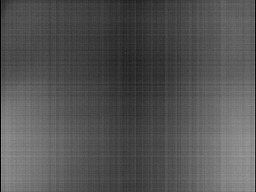
\includegraphics[height=5cm]{images/blackframes-gainx1-offset2047-5ms-01}
\end{center}

\begin{center}
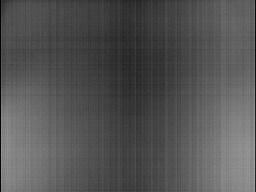
\includegraphics[height=5cm]{images/darkavg-5ms}
\end{center}

What about camera settings?\\

Unfortunately, dark frames depend on many camera settings: analog gain (ISO), exposure, other sensor settings like offset, black sun protection, PLR configuration and so on. Temperature is a variable as well.\\

Luckily, the dependence on exposure appears to be linear, so we can take calibration frames at various exposures, combine them into a single dark frame, adjust it for the dark current and use it for the entire range of exposure settings (hopefully). We'll discuss that in the next section.\\ 

\textbf{Dark current}\\

Let's look at some dark frames: gain x1, exposures 1.2ms, 6ms and 78ms. Notice they get brighter as exposure increase.\\

\begin{center}

\includegraphics[height=5cm]{images/blackframes-gainx1-offset2047-1ms-01}
\end{center}

\begin{center}
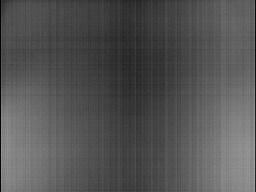
\includegraphics[height=5cm]{images/darkavg-5ms}
\end{center} 

\begin{center}
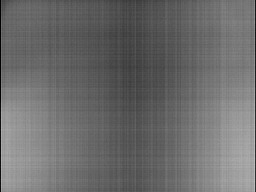
\includegraphics[height=5cm]{images/blackframes-gainx1-offset2047-64ms-01}
\end{center}

The overall brightness in the dark frame changes with exposure in a linear fashion. We'll try to account for this in two ways: with a simple scalar value, and with a per-pixel correction.\\

The values in the black reference columns do not appear to compensate for the dark current, so we'll need to do it ourselves.\\

By identifying the dark current, we will be able to compute a dark frame that is applicable to any usual exposure time, but we are going to store only one or two reference frames for each gain. First reference frame will be called a bias frame (a zero-length exposure, that would contain only static black offsets), and the second reference frame, if used, will be called a dark current frame.\\

Dark current cannot be fully corrected because, while its stationary value can be measured and subtracted, it also introduces photon noise. Roger Clark explains it better:\\ 

\textit{"Dark current is temperature dependent and most modern CMOS digital cameras, circa 2008 and later have on sensor dark current subtraction, but while the dark current level is subtracted, the noise from the dark current still accumulates."} - Source: \href{http://www.clarkvision.com/reviews/how-to-interpret-reviews/}{http://www.clarkvision.com/reviews/how-to-interpret-reviews/}

\textbf{Simple correction}\\

Experimentally, we have found the dark frame changes with exposure at roughly 0.065 digital units for each ms. This value is multiplied by analog gain. To find this value, take the dark frames at different exposure times (say 1...50 ms), then do a linear fit for the frame average (or median).\\

Command-line:

\consolecommand{raw2dng *x1*.raw12 --calc-darkframe}

Example: a dark frame created from 256 exposures, between 1.2ms and 77ms, without using black reference columns. The image was adjusted (with a constant offset) to match a zero-length exposure, so calling it bias frame may be a good idea. If we use it to correct the individual dark frames, we should no longer see a variation in overall brightness. 

\consolecommand{    Averaged 256 frames exposed from 1.19 to 76.79 ms.
    Dark current: 0.0653 DN/ms}
    
Image sequence: bias frame, single dark frames at exposures 1.2, 6 and 77 ms, corrected with the bias frame and the (scalar) dark current average. All files scaled to show a range of 60 DN, but the master dark frame has a different offset than the others.     


\begin{center}
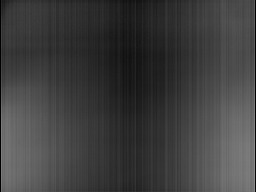
\includegraphics[height=5cm]{images/darkframe-x1-no-blackcol-256}
\end{center}

\begin{center}

\includegraphics[height=5cm]{images/blackframes-gainx1-offset2047-1ms-01-simple-darkframe-no-blackcol}
\end{center} 

\begin{center}

\includegraphics[height=5cm]{images/blackframes-gainx1-offset2047-5ms-01-simple-darkframe-no-blackcol}
\end{center}

\begin{center}

\includegraphics[height=5cm]{images/blackframes-gainx1-offset2047-64ms-01-simple-darkframe-no-blackcol}
\end{center}





\paragraph{Dark Current Non-uniformity Correction}

One common use of bias frames is for scaling dark frames. By subtracting a bias frame from a dark frame, you end up with a thermal frame. A thermal frame contains pixel values showing just the effect of dark current. Because dark current in any given pixel accumulates at a constant rate, a thermal frame allows you to predict with reasonable accuracy how much dark current there would be for different length exposures. However, given the opportunity, you’re always better off taking dark frames that match the exposure times of your light frames.\\

\href{http://qsimaging.com/ccd_noise_measure.html}{http://qsimaging.com/ccd\_noise\_measure.html}{Source}: \\

\textit{"Dark current non-uniformity is a noise that results from the fact that each pixel generates a slightly different amount of dark current. This noise can be eliminated by subtracting a dark reference frame from each image. The dark reference frame should be taken at the same temperature and with the same integration time as the image."} - Source: \href{https://www.photometrics.com/resources/learningzone/darkcurrent.php}{https://www.photometrics.com/resources/learningzone/darkcurrent.php}\\

\textit{"Dark noise is not random; in fact, it is highly repeatable. A given photosite on a sensor will accumulate almost exactly the same amount of dark noise from one exposure to the next, as long as temperature and exposure duration do not vary."}\\

So, rather than using a single scalar value (0.06 dn/ms/gain) for all pixels, we can try finding the individual dark current for each pixel. Instead of doing a linear fit on the overall dark frame brightness (vs exposure), we will do the linear fit per pixel. We'll have to acquire a lot more dark frames to compute a good result, but it might be worth the trouble.\\

Command-line:\\

\consolecommand{raw2dng *x1*.raw12 --calc-dcnuframe}

Example: bias frame (static offset) and dark current frame (exposure-dependent offset). Notice the bias frame looks quite similar to the previous one, but a little darker. The median value of the dark current frame is, unsurprisingly, 0.0645 DN/ms. 

\begin{center}

\includegraphics[height=5cm]{images/darkframe-x1-no-blackcol-darkcurrent-256}
\end{center}

\begin{center}
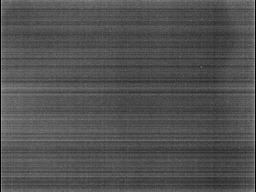
\includegraphics[height=5cm]{images/dcnuframe-x1-no-blackcol-darkcurrent-256}
\end{center}

Individual dark frames (1.2, 6 and 77 ms) adjusted with dark current nonuniformity: 

\begin{center}

\includegraphics[height=5cm]{images/blackframes-gainx1-offset2047-1ms-01-darkcurrent-no-blackcol}
\end{center}

\begin{center}

\includegraphics[height=5cm]{images/blackframes-gainx1-offset2047-5ms-01-darkcurrent-no-blackcol}
\end{center}

\begin{center}

\includegraphics[height=5cm]{images/blackframes-gainx1-offset2047-64ms-01-darkcurrent-no-blackcol}
\end{center}

No obvious improvement in the test images, so why bother?\\

Let's correct all these 256 dark frames and check a few indicators: median, stdev, row noise and column noise.\\ 

Dark frame + scalar dark current: 
\begin{center}
\includegraphics[height=5cm]{images/darkframe-check-x1-256-simple}
\end{center}


Dark frame + dark current frame:
\begin{center}
\includegraphics[height=5cm]{images/darkframe-check-x1-256-dcnu}
\end{center}

You may notice:\\

- Median (black level) variation: noticeable improvement with the second method.\\
- stdev (overall noise): minor improvement at extreme settings.\\
- Row noise: identical with both methods.\\
- Column noise: small improvement with the second method.\\

Indeed, the more complex method appears just a tiny bit better than the simpler one.\\





\paragraph{Dark Current Measurement From Hot Pixels}

A very interesting idea can be found here - \href{https://www.photonics.com/Article.aspx?AID=44298}{https://www.photonics.com/Article.aspx?AID=44298} ... where hot pixels can be used to measure the amount of dark current and scale it properly. This will probably account for changes in temperature, and may work at very long exposures without actually having to calibrate the camera in these conditions. Genius, if you ask me. 





\paragraph{Black Reference Columns}

This sensor has 8+8 columns that can be used for calibrating the black levels; they are also useful for reducing the dynamic row noise.\\

Experimentally, we have noticed that odd rows have slightly different statistics (noise level, offset, gain), compared to even rows. This happens in both the black columns and the active area, and it may indicate two parallel circuits used for readout, each having slightly different electrical response.\\

Therefore, it may be wise to process the black columns for odd and even rows separately, which should already fix some issues like static row noise, or the need for green equilibration.\\

In raw2dng, this correction is enabled by default, as long as you use a dark frame. You can turn it off with \importantKeyword{--no-blackcol}, if you want. \\





\paragraph{Black Level}

The sensor has two registers that can be used to adjust the black level: one for odd rows, another for even rows. This confirms our finding about two parallel readout circuits.\\

You might be tempted to adjust the black level to 0 (like Nikon does). Please don't. Here's why:\\

- If you adjust the offset until the black level becomes roughly 0, you will clip all the data below this level. Good luck subtracting a dark frame after that.\\
- Even if you change the level after doing all the black corrections, you may still have useful data below zero. You will need it when stacking multiple frames, or when doing noise reduction.\\

Just FYI, there is a hack for Nikon cameras that moves the black level above 0. See \href{https://landingfield.wordpress.com/2014/05/13/teaser-nikon-dslr-black-point-hack-for-astrophotography/}{https://landingfield.wordpress.com/2014/05/13/teaser-nikon-dslr-black-point-hack-for-astrophotography/} \\

... Sample photos can be found \href{https://www.cloudynights.com/topic/473696-rho-ophiuchi-with-nikon-hacked-black-level/}{here} or \href{https://nikonhacker.com/viewtopic.php?t=2548&p=18449#p17973}{here}.

We recommend setting the offset so that only a few isolated pixels (if any) reach the value of 0. A black offset of 2047 (registers 87/88) is a good choice. You won't lose any dynamic range by doing that.\\

On most recent Canon DSLRs, black level is 2048. That's a little on the large side, but it's a good thing. Some may argue that you may lose 2 stops or more of dynamic range by doing that (reading - \href{https://www.reddit.com/r/photography/comments/3q4tnz/how_to_correctly_push_5_stops_with_canon/cwcbyb5/}{https://www.reddit.com/r/photography/comments/3q4tnz/how\_to\_correctl\_push\_5\_stops\_with\_canon/cwcbyb5/} ), but this is wrong. On Canons, the raw output is 14-bit, so by setting the offset to 2048 instead of 0, the useful range will be "just" log2(16384-2048) = 13.8 bits, instead of 14. So, yeah, you lose 0.2 bits from the ADC range.\\

With the black offset of 2047 on the CMV12K, the black level ends up at around 150, so you lose a whooping 0.05 bits from the 12-bit range.\\

\textbf{Note:} for easier processing, raw2dng shifts the raw data in order to fix the black level at 128.\\

\textbf{Note also:} Row noise correction from black columns detailed in 11.2 Pattern Noise.
 




\subsubsection{Checking Black Level}

You may wonder: after all these corrections, did we get the right black level? Can we render shadow detail correctly?\\

A possible criteria for checking: if we have two images of the same scene, taken with different exposures, we should be able to match those in postprocessing by simply dragging the exposure slider. For example, if we have one image at 5ms and another one at 20ms, we would set the exposure to +2 EV on the first image - the results should be pretty much identical, except for noise (and clipped highlights, if we weren't careful with the exposure). \\

Of course, that will work once we know the sensor Response Curves (See 11.5).\\

To check how well the images can be exposure-compensated, we could evaluate (and minimize) one of those error metrics: 

\begin{lstlisting}[language=bash,morekeywords=$,keywordstyle=\bfseries,frame=none,xleftmargin=.25in,belowskip=2em, aboveskip=2em]
    a  = dark\_image - black\_level;
    b  = bright\_image - black\_level;
    e1 = norm(a*expo\_ratio - b);
    e2 = abs(median((b ./ a)(:)) - expo\_ratio)
    e3 = mad(log2((b ./ a)(:)));
\end{lstlisting}

First metric checks the difference between the two images, where the darkest one was adjusted by scaling (gain) to match the brightest one. Second metric computes the ratio between the two images at each pixel, and checks its median value vs the expected value. Third one checks the variation of per-pixel ratios between the two images, in stops, ignoring the expected value - this metric could be useful if we suspect the exposure controls may not be accurate.\\

\begin{center}
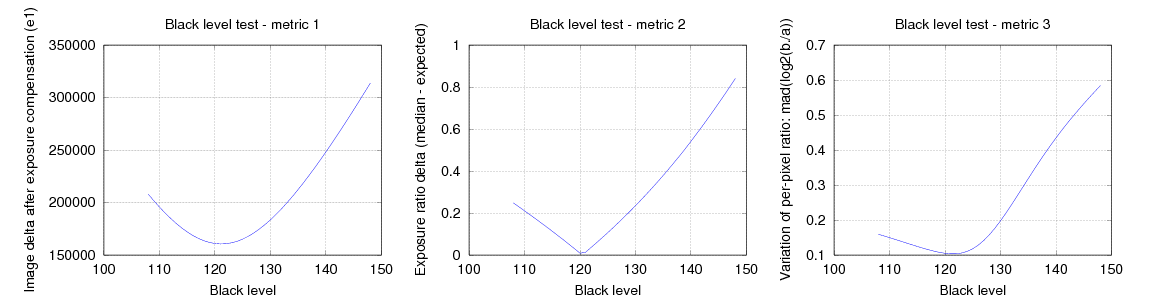
\includegraphics[height=5cm]{images/black_check}
\end{center}

With all 3 methods, minimization indicates a black level of around 120-122 (expected 128), so there's still something missing with our calibration. This is confirmed by missing details in very dark areas (crushed blacks) on some sample images.\\ 

On the same test image, the response curve estimated from the grayscale IT8 reference data indicates a black level of 129. 

On the same test image, the response curve estimated with the Robertson02 algorithm indicates a black level of 124 (See 11.5).\\

Who is right?\\

The sensor also has a strange behavior - something we have called the "Black Hole" anomaly: in very dark areas, sensor output decreases with exposure time. This might give a clue for solving this mystery.\\

\begin{center}
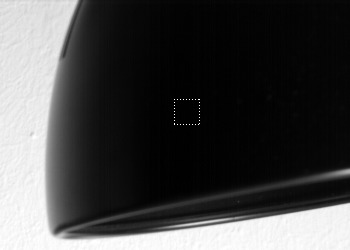
\includegraphics[height=5cm]{images/blackhole}
\end{center}





\subsubsection{Calibration Pipeline}

- Use black reference columns to find the black levels for odd and even rows.\\
- Subtract dark offset and dark current.\\
- Use variations in black reference columns to reduce row noise.\\ 

These operations should be simple enough to be implemented in FPGA, as real-time corrections. 





\subsubsection{Calibration Procedure}

\textbf{Quick calibration}\\

Acquire 16 dark frames, gain x1, exposures between 1 and 50 ms, save them under the 'darkframes' subdirectory, then run: 

\consolecommand{raw2dng darkframes/*x1*.raw12 --calc-darkframe --swap-lines}

Result: darkframe-x1.pgm.\\

Repeat for other gains if needed.\\ 


\textbf{Accurate calibration, with dark current nonuniformity}

Acquire 256 dark frames, gain x1, exposures between 1 and 64 ms in linear increments (4 images at each setting), save them under the 'darkframes' subdirectory, then run: 

\consolecommand{raw2dng darkframes/*x1*.raw12 --calc-dcnuframe --swap-lines}

Result: darkframe-x1.pgm and dcnuframe-x1.pgm.\\

Repeat for other gains if needed. \\

\textbf{Checking the calibration}\\

You can verify the calibration by rendering the same individual dark frames, this time corrected, to check the residuals. Or, even better, acquire a new set of dark frames at the same settings, and check those instead: 

\consolecommand{raw2dng darkframes/*x1*.raw12 --check-darkframe --swap-lines}

You will see the average value, pixel noise and row/column noise levels (both absolute and relative to pixel noise) for each dark frame. Example:

\consolecommand{    Average     : 127.48
    Pixel noise : 2.48
    Row noise   : 0.61 (24.6%)
    Col noise   : 0.05 (2.2%)}
    
Using the reference frames to correct raw12 files.\\

1. Place the calibration files in the working directory.\\
2. Make sure your \importantKeyword{.raw12} images contain a metadata block.\\
3. raw2dng will recognize the dark frames and use them for correcting your image. \\
   
\consolecommand{    cp /path/to/darkframes/*-x[1-4].pgm .
    raw2dng *.raw12 --swap-lines}
    
\textbf{Note:} you need --swap-lines as an workaround for an old bug introduced in the Beta, but wasn't fixed yet in the FPGA.\\    
    
This is not exactly useful when dealing with multiple folders, so until we'll have a better way to organize the calibration frames, you may try an alternative workflow:\\

1. Place the calibration files in some directory (let's call it "calibration directory")\\.
2. Make sure your .raw12 images contain a metadata block.\\
3. Use paths when passing input files raw2dng (the output files will be saved in the same directory as the input file).\\

\consolecommand{    cd /path/to/darkframes
    ls *.pgm
      darkframe-x1.pgm       dcnuframe-x1.pgm       ...
    raw2dng /path/to/images/*.raw12 --swap-lines}
     
    
\textbf{Example}

Showing half-res image crops pushed by 4 stops (ufraw-batch --wb=auto --exposure=4 --shrink=2).

- Top left: raw sensor data (adjusted black level manually).\\
- Top right: corrected with dark frame, scalar dark current, no black columns.\\
- Bottom left: corrected with dark frame, dark current frame, no black columns.\\
- Bottom right: corrected with dark frame, dark current frame, black columns enabled.\\

\textbf{Note:} in the raw data, even and odd rows have different black offsets; that's why we have wrong colors. \\

\begin{center}
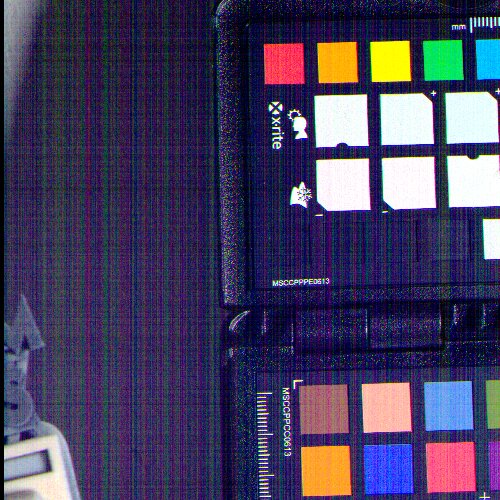
\includegraphics[height=5cm]{images/10ms+4-totally-raw-crop}
\end{center}

\begin{center}
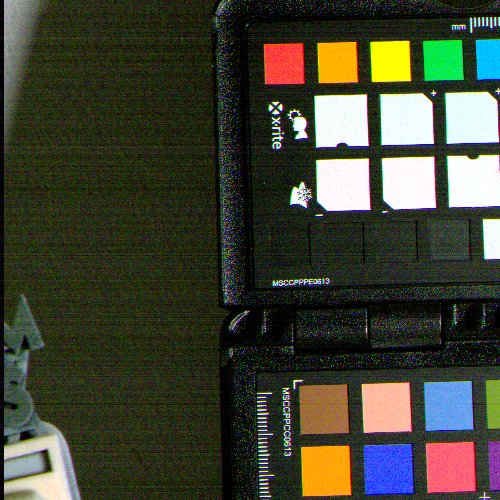
\includegraphics[height=5cm]{images/10ms+4-no-blackcol-crop}
\end{center}

\begin{center}
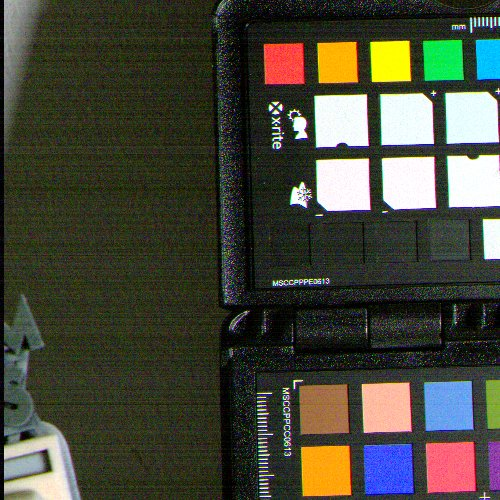
\includegraphics[height=5cm]{images/10ms+4-darkcurrent-no-blackcol-crop}
\end{center}

\begin{center}
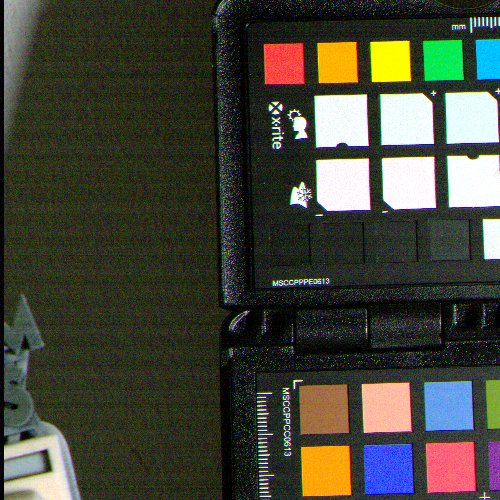
\includegraphics[height=5cm]{images/10ms+4-darkcurrent-crop}
\end{center}


    

\subsection{Pattern Noise}

General info about pattern noise can be found here - \href{http://theory.uchicago.edu/~ejm/pix/20d/tests/noise/#patternnoise}{http://theory.uchicago.edu/~ejm/pix/20d/tests/noise/#patternnoise} \\

The CMV12000 sensor suffers from dynamic row noise.\\

That means, a scalar offset gets added to each row. The offset is not correlated between different frames, so we can't remove it using a calibration frame (dark frame or whatever).\\

One can observe this noise by looking at the difference between two images taken at identical settings. There are two main components that appear obvious in such a difference frame: random noise (per pixel, increases on brighter pixels) and row noise (per line). \\

\begin{center}
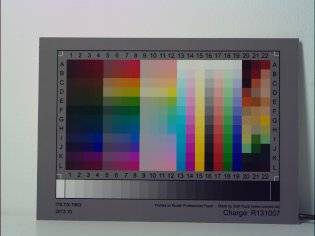
\includegraphics[height=5cm]{images/it8-gainx1-offset2047-20ms-01}
\end{center}

\begin{center}
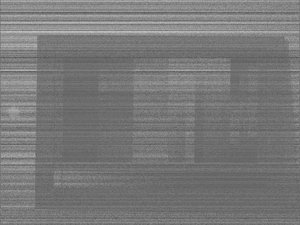
\includegraphics[height=5cm]{images/it8-gainx1-offset2047-20ms-01-minus-02-small}
\end{center}




\subsubsection{Correction Methods}

There are two ways to deal with this noise, after performing Black Calibration (See 11.1)\\

- Use info from black reference columns to reduce dynamic row noise without guessing anything (fast, can be implemented in real-time, see Raw Preprocessing).\\
- Use denoising techniques to reduce the remaining row noise (the guesswork part, slow).\\

\textbf{Reducing row noise using black reference columns}

See \href{http://github.com/apertus-open-source-cinema/misc-tools-utilities/commit/48de47b2a544dc32bbd5a8fd7701bb44a31ea850#diff-624053a553f49c0036b4d31282e58b2fR301}{http://github.com/apertus-open-source-cinema/misc-tools-utilities/commit/48de47b2a544dc32bbd5a8fd7701bb44a31ea850#diff-624053a553f49c0036b4d31282e58b2fR301}

The application note AN01 from CMOSIS says:\\

\textit{"The noise is also present in the black reference columns (8 left and 8 right), so when enabled (reg 89[15] = 1), these can be used for row noise correction by for example making a relative row profile of these black columns and subtract this from the image."}\\

However, simply subtracting each row average of the black columns from our image is not going to work. Here's why:\\

Kalman filter theory: \href{http://robocup.mi.fu-berlin.de/buch/kalman.pdf}{http://robocup.mi.fu-berlin.de/buch/kalman.pdf} \\

From page 3, if we know how noisy our estimations are, the optimal weights are inversely proportional with the noise variances:\\

\consolecommand{x\_optimal = (x1 * var(x2) + x2 * var(x1)) / (var(x1) + var(x2))} 

Here, let's say R = x1 is row noise (stdev = 1.6 at gain=x1) and x2 is black column noise. 

\begin{lstlisting}[language=bash,morekeywords=$,keywordstyle=\bfseries,frame=none,xleftmargin=.25in,belowskip=2em, aboveskip=2em]
    R = x1
    B = mean(black\_col') = R + x2 =>  x2 = B - R
    x2 can be estimated as mean(black\_col') - mean(active\_area')
    stdev(x2) = 1.3.
\end{lstlisting}

We want to find k that minimizes var(R - k*B). 

\begin{lstlisting}[language=bash,morekeywords=$,keywordstyle=\bfseries,frame=none,xleftmargin=.25in,belowskip=2em, aboveskip=2em]
    var(R - k*B) = var(x1 * (1-k) - x2 * k),
    => k = var(x1)) / (var(x1) + var(x2).
\end{lstlisting}

In particular, for gain = x1, k = 1.6^2 / (1.6^2 + 1.3^2) = 0.6.\\

So, we don't have to simply subtract the black columns. Rather, we'll subtract the static offset (median value) first, and then, we'll subtract the remaining variations multiplied by 0.6 at gain=x1.\\

Things get a little more complex because the static offset is different on odd and even rows, and it also appears to change from the left side to right side of the frame. More details on the \textbf{Raw Preprocessing} page.\\

\textbf{Fixed frequency perturbation in black columns }\\

A closer look at the frequency spectrum of the black columns, compared to the spectrum of the row noise from a dark frame, revealed a strong fixed-frequency component present only in the black columns. Attempting to fix row noise with the above procedure would introduce some of this fixed frequency component in the main image as well.\\

In the example image from below, this component has a frequency of 1/41.27 pixels-1, with an amplitude of 1.14 DN. The value is different in other test images, and appears to be consistent in the images taken during the same experiment. It doesn't change with exposure time. Cause is unknown. \\

TODO: detailed analysis, FFT graphs...\\

We'll attempt to filter out this perturbation from the black columns before using them for reducing row noise.\\

Good news: after removing this perturbation, the optimal black columns multiplier increases to about 0.8 :) \\

\textbf{Using nearby rows to reduce the row noise even more}\\

Maybe some nearby rows could offer some hints about the row offset on the line being analyzed?\\

Looks like yes. Trying to write the row noise as a linear combination of row averages from black columns, using linear regression, not just the ones from the same row, but also from nearby rows, and discarding very small coefficients, gives the following filter:\\

 \begin{lstlisting}[language=bash,morekeywords=$,keywordstyle=\bfseries,frame=none,xleftmargin=.25in,belowskip=2em, aboveskip=2em]
    (y % 2)
       ?
         black\_col[y-1] *  0.24 +
         black\_col[y]   *  0.63
       :
         black\_col[y]   *  0.38 +
         black\_col[y+1] *  0.43
\end{lstlisting}

What's interesting: on even rows, row noise (in the active area) depends on the black column average from the same row, but also on the black column average from the previous row. But on odd rows, it depends on the black column average from the same row and the next row. This probably means they are processed in pairs, and there is some common perturbation that affects both of them.\\

This gives a minor improvement (0.6 -> 0.5). \\

\textbf{Exploiting differences in green channels}

The two green channels are expected to be nearly identical, except for high-frequency details like sharp edges. That means, if we take the median difference on each row, we expect to get zero. In practice, we get some nonzero values. We could try to see if there is any correlation between those green channel differences and our row noise.\\

Let's extract only the green channels from an image: the result will be W x H/2. Let's define green_delta(lag) = row_median(green - circshift(green,-lag)). That means, from each green row, subtract some nearby green row, and take the median difference. We'll compute this at lags -2, -1, 1, 2, mapped to array indices 0, 1, 2, 3.\\

Linear regression gives an ugly FIR filter that looks like this: \\

\begin{lstlisting}[language=bash,morekeywords=$,keywordstyle=\bfseries,frame=none,xleftmargin=.25in,belowskip=2em, aboveskip=2em]
    (y % 2)
       ?
         black\_col[y-2]    * 0.17 +
         black\_col[y-1]    * 0.14 +
         black\_col[y+0]    * 0.17 +
         black\_col[y+1]    * 0.16 +
         black\_col[y+2]    * 0.14 +
         green\_delta[0][y] * 0.22 +
         green\_delta[1][y] * 0.31 +
         green\_delta[2][y] * 0.38
       :
         black\_col[y-2]    * 0.12 +
         black\_col[y-1]    * 0.13 +
         black\_col[y+0]    * 0.14 +
         black\_col[y+1]    * 0.14 +
         black\_col[y+2]    * 0.12 +
         black\_col[y+3]    * 0.12 +
         green\_delta[0][y] * 0.33 +
         green\_delta[3][y] * 0.32
\end{lstlisting}

As weird as it looks, it seems to work!\\

Improvement (over the "Kalman" scaling of black columns): 0.6 -> 0.3.\\ 



\textbf{Reducing the remaining row noise by image filtering}\\

Basic algorithm:\\

1. Filter the image with an edge-aware vertical blur (bilateral filter on pixels from the same column)\\
2. Subtract the blurred image; the residuals will reveal the row noise (see example)\\
3. Mask out highlights and strong edges\\
4. Take the median value from each row of the residuals image\\
5. Subtract these values from each row of the original image \\

Source: \href{https://github.com/apertus-open-source-cinema/misc-tools-utilities/blob/master/raw2dng/patternnoise.c}{https://github.com/apertus-open-source-cinema/misc-tools-utilities/blob/master/raw2dng/patternnoise.c} \\





\subsubsection{Usage}

The methods discussed here are implemented here = \href{https://github.com/apertus-open-source-cinema/misc-tools-utilities/tree/master/raw2dng}{https://github.com/apertus-open-source-cinema/misc-tools-utilities/tree/master/raw2dng} \\

- Black reference columns are used by default, as long as you use a dark frame (since this method is fast and has no side effects)\\
- To reduce the remaining row noise, use \importantKeyword{raw2dng --fixrn}\\
- If the image also suffers from column noise, use \importantKeyword{raw2dng --fixpn} \\

Troubleshooting or checking the effectiveness of each step:

- Disable row noise reduction from black columns, but use the static offsets: \importantKeyword{--no-blackcol-rn}\\
- Disable fixed frequency correction for black columns: \importantKeyword{--no-blackcol-ff}\\
- Disable black reference columns completely: \importantKeyword{--no-blackcol} (you need to compute new darkframes if you use this)\\ 

Tip: the algorithm for filtering row noise is also available in MLVFS, so you can use it on MLV videos (recorded with Magic Lantern) as well. See - \href{http://www.magiclantern.fm/forum/index.php?topic=13152}{http://www.magiclantern.fm/forum/index.php?topic=13152}





\subsubsection{Tests on a dark frame}

Checking a single 10ms dark frame, corrected using 256 exposures between 1.2ms and 77ms, various settings. Showing only noise measurements.

\begin{lstlisting}[language=bash,morekeywords=$,keywordstyle=\bfseries,frame=none,xleftmargin=.25in,belowskip=2em, aboveskip=2em]
    # raw data without any processing
    raw2dng blackframes-gainx1-offset2047-10ms-01.raw12 --swap-lines --no-darkframe --check-darkframe
      Average     : 190.35
      Pixel noise : 7.14
      Row noise   : 5.29 (74.1%)
      Col noise   : 5.41 (75.7%)
\end{lstlisting}

\begin{lstlisting}[language=bash,morekeywords=$,keywordstyle=\bfseries,frame=none,xleftmargin=.25in,belowskip=2em, aboveskip=2em]
    # disable black columns, simple darkframe
    raw2dng *x1*.raw12 --calc-darkframe --no-blackcol --swap-lines
    raw2dng blackframes-gainx1-offset2047-10ms-01.raw12 --swap-lines --no-blackcol --check-darkframe
      Average     : 140.33
      Pixel noise : 3.08
      Row noise   : 1.33 (43.0%)
      Col noise   : 0.09 (3.0%)
\end{lstlisting}

\begin{lstlisting}[language=bash,morekeywords=$,keywordstyle=\bfseries,frame=none,xleftmargin=.25in,belowskip=2em, aboveskip=2em]
    # disable black columns, enable dark current frame
    raw2dng *x1*.raw12 --calc-dcnuframe --no-blackcol --swap-lines
    raw2dng blackframes-gainx1-offset2047-10ms-01.raw12 --swap-lines --no-blackcol --check-darkframe
      Average     : 142.46
      Pixel noise : 3.06
      Row noise   : 1.32 (43.1%)
      Col noise   : 0.08 (2.5%)
\end{lstlisting}

\begin{lstlisting}[language=bash,morekeywords=$,keywordstyle=\bfseries,frame=none,xleftmargin=.25in,belowskip=2em,     # dark current frame, use only static offsets from black columns
    raw2dng *x1*.raw12 --calc-dcnuframe --swap-lines
    raw2dng blackframes-gainx1-offset2047-10ms-01.raw12 --swap-lines --no-blackcol-rn --check-darkframe
      Average     : 127.46
      Pixel noise : 3.06
      Row noise   : 1.39 (45.4%)
      Col noise   : 0.10 (3.2%)
\end{lstlisting}

\begin{lstlisting}[language=bash,morekeywords=$,keywordstyle=\bfseries,frame=none,xleftmargin=.25in,belowskip=2em, aboveskip=2em]
    # dark current frame, enable black columns, don't remove the fixed frequency component from black columns
    raw2dng blackframes-gainx1-offset2047-10ms-01.raw12 --swap-lines --no-blackcol-ff --check-darkframe
      Average     : 127.46
      Pixel noise : 2.90
      Row noise   : 0.82 (28.2%)
      Col noise   : 0.10 (3.3%)
\end{lstlisting}

\begin{lstlisting}[language=bash,morekeywords=$,keywordstyle=\bfseries,frame=none,xleftmargin=.25in,belowskip=2em, aboveskip=2em]
    # dark current frame, enable black columns, remove the fixed frequency component (default setting)
    raw2dng blackframes-gainx1-offset2047-10ms-01.raw12 --swap-lines --check-darkframe
      Average     : 127.46
      Pixel noise : 2.85
      Row noise   : 0.61 (21.4%)
      Col noise   : 0.10 (3.4%)
\end{lstlisting}

\begin{lstlisting}[language=bash,morekeywords=$,keywordstyle=\bfseries,frame=none,xleftmargin=.25in,belowskip=2em, aboveskip=2em]
    # also enable --fixrn (aggressive correction)
    raw2dng blackframes-gainx1-offset2047-10ms-01.raw12 --swap-lines --fixrn --check-darkframe
      Average     : 127.42
      Pixel noise : 2.79
      Row noise   : 0.12 (4.1%)
      Col noise   : 0.10 (3.5%)
\end{lstlisting}

So, row noise was reduced from 1.33 (after dark frame correction) to 0.61 after using the black reference columns.\\

If it's still noticeable, \importantKeyword{--fixrn} should bring it to very low levels, unless you have strong horizontal lines in the image, which might trick the algorithm.\\

Some experimental row noise filters:\\

\begin{lstlisting}[language=bash,morekeywords=$,keywordstyle=\bfseries,frame=none,xleftmargin=.25in,belowskip=2em, aboveskip=2em]
    % 2-tap FIR, separate for odd/even rows
    raw2dng blackframes-gainx1-offset2047-10ms-01.raw12 --swap-lines --rnfilter=1 --check-darkframe
      Average     : 127.44
      Pixel noise : 2.84
      Row noise   : 0.51 (18.1%)
      Col noise   : 0.10 (3.4%)
\end{lstlisting}

\begin{lstlisting}[language=bash,morekeywords=$,keywordstyle=\bfseries,frame=none,xleftmargin=.25in,belowskip=2em, aboveskip=2em]
    % that ugly FIR that also looks at green channel differences
    raw2dng blackframes-gainx1-offset2047-10ms-01.raw12 --swap-lines --rnfilter=2 --check-darkframe
      Average     : 127.47
      Pixel noise : 2.81
      Row noise   : 0.31 (11.1%)
      Col noise   : 0.10 (3.4%)
\end{lstlisting}


\textbf{Example}

Showing half-res image crops pushed by 4 stops (ufraw-batch --wb=auto --exposure=4 --shrink=2).\\


- Left: raw sensor data (adjusted black level manually).\\
- Right: after dark frame and dark current subtraction, but without correction from black columns.\\
- Note: in the raw data, even and odd rows have different black offsets; that's why we have wrong colors.\\ 

\begin{center}
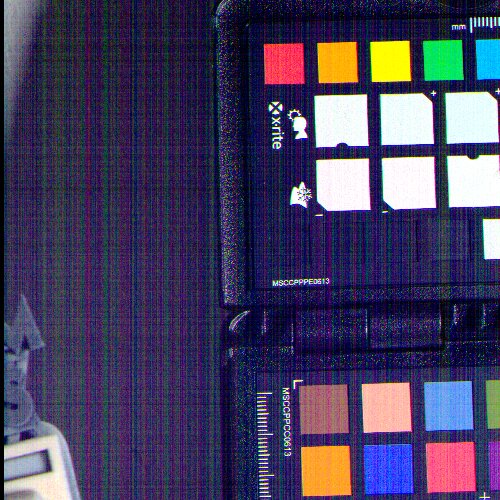
\includegraphics[height=5cm]{images/10ms+4-totally-raw-crop}
\end{center}

\begin{center}
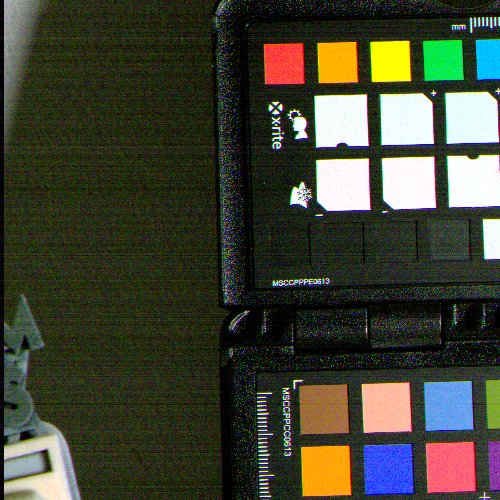
\includegraphics[height=5cm]{images/10ms+4-no-blackcol-crop}
\end{center}

- Left: after dark frame, dark current and static offsets from black reference columns.\\
- Right: after dark frame, dark current and black reference columns correction, without removing the fixed frequency component.\\

 \begin{center}
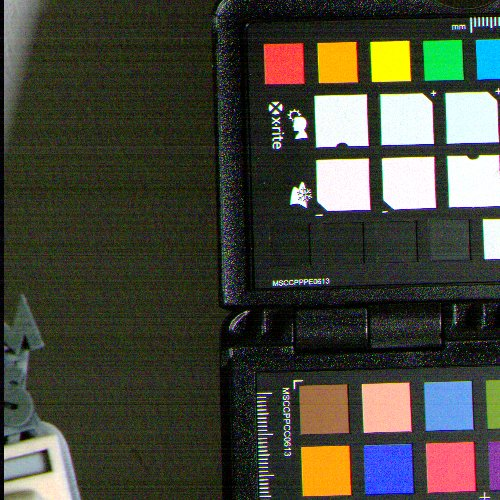
\includegraphics[height=5cm]{images/10ms+4-no-blackcol-rn-crop}
\end{center}

\begin{center}
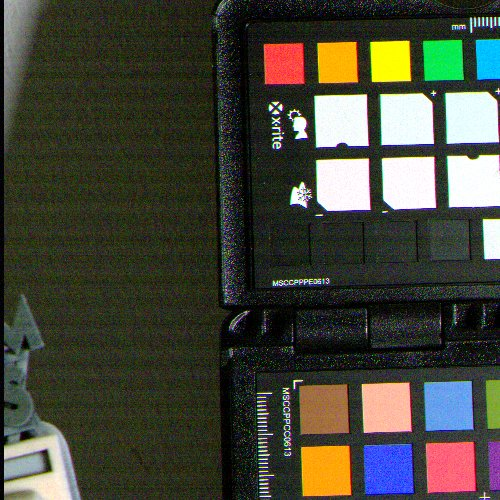
\includegraphics[height=5cm]{images/10ms+4-no-blackcol-ff-crop}
\end{center}

- Left: after dark frame, dark current and black reference columns correction.\\
- Right: after row noise reduction \importantKeyword{--fixrn} \\

\begin{center}
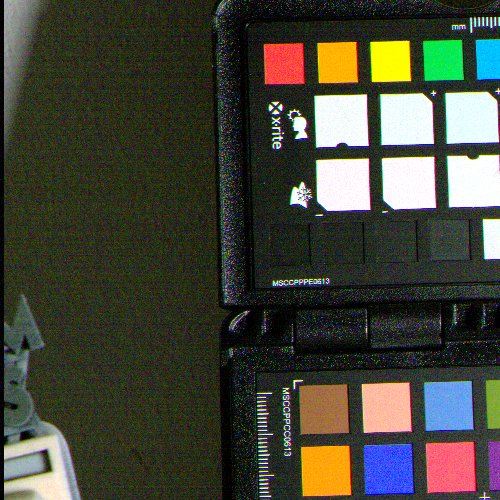
\includegraphics[height=5cm]{images/10ms+4-crop}
\end{center}

\begin{center}
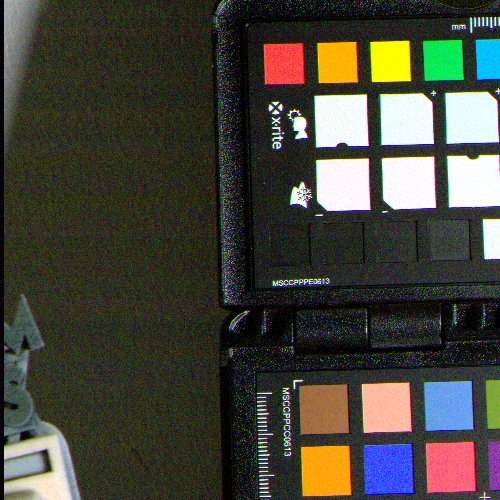
\includegraphics[height=5cm]{images/10ms+4-fixrn-crop}
\end{center}

- Left: \importantKeyword{--rnfilter=1} \\
- Right: \importantKeyword{--rnfilter=2} \\

\begin{center}
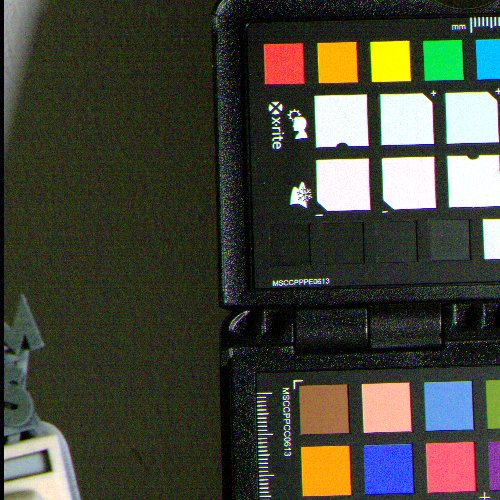
\includegraphics[height=5cm]{images/10ms+4-rnfilter1-crop}
\end{center}

\begin{center}
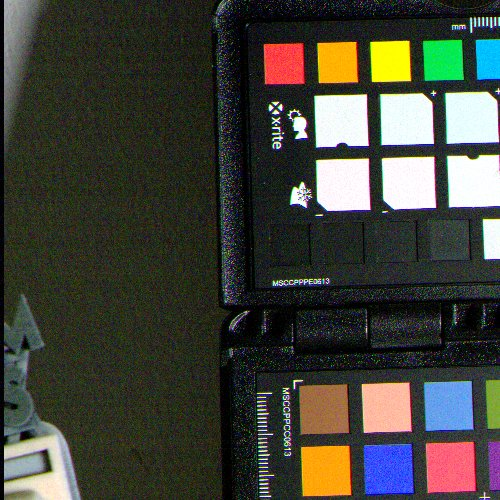
\includegraphics[height=5cm]{images/10ms+4-rnfilter2-crop}
\end{center}

Algorithm internals for \importantKeyword{--fixrn}

- Left: filtered image (vertical blur using a bilateral filter)\\
- Right: noise image, revealing row noise. Black regions are from edges that were masked.\\ 

\begin{center}
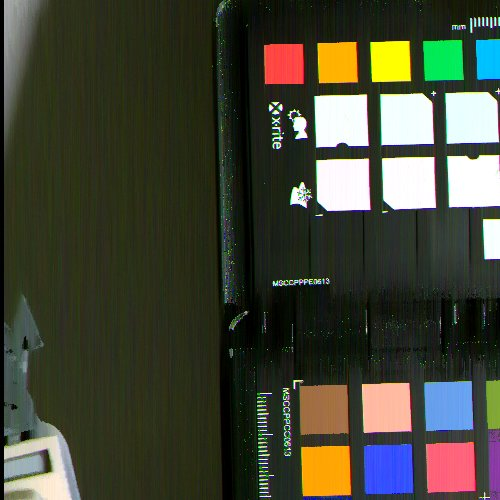
\includegraphics[height=5cm]{images/10ms+4-fixrn-dbg-denoised-crop}
\end{center}

\begin{center}
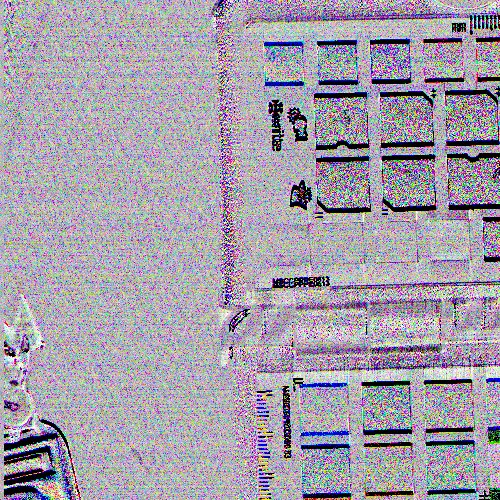
\includegraphics[height=5cm]{images/10ms+4-fixrn-dbg-noise-crop}
\end{center}

\textbf{Downsized images}\\

Corrected with dark frame and dark current only:\\
 
\begin{center}
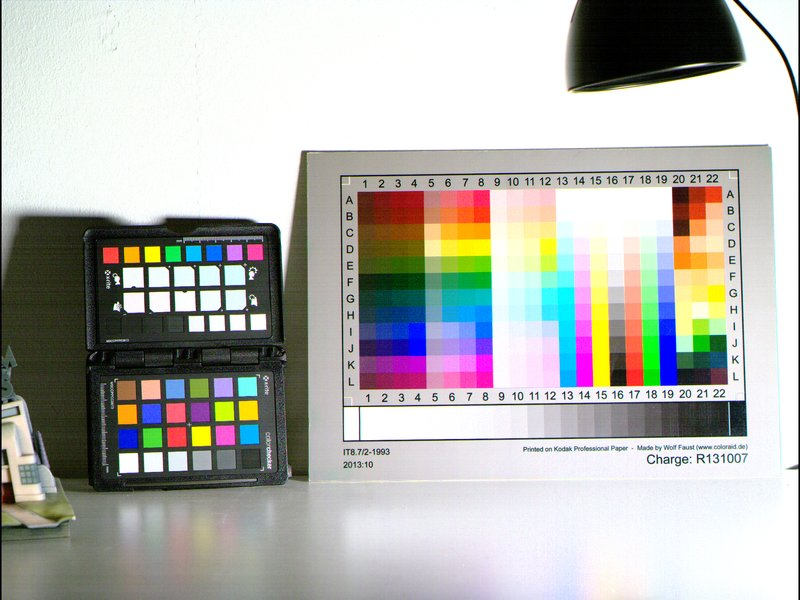
\includegraphics[height=5cm]{images/10ms+4-no-blackcol-small}
\end{center}

Also corrected with black columns: 

\begin{center}
\includegraphics[height=5cm]{images/10ms+4-smallp}
\end{center}

Also corrected with \importantKeyword{--fixrn} 

\begin{center}
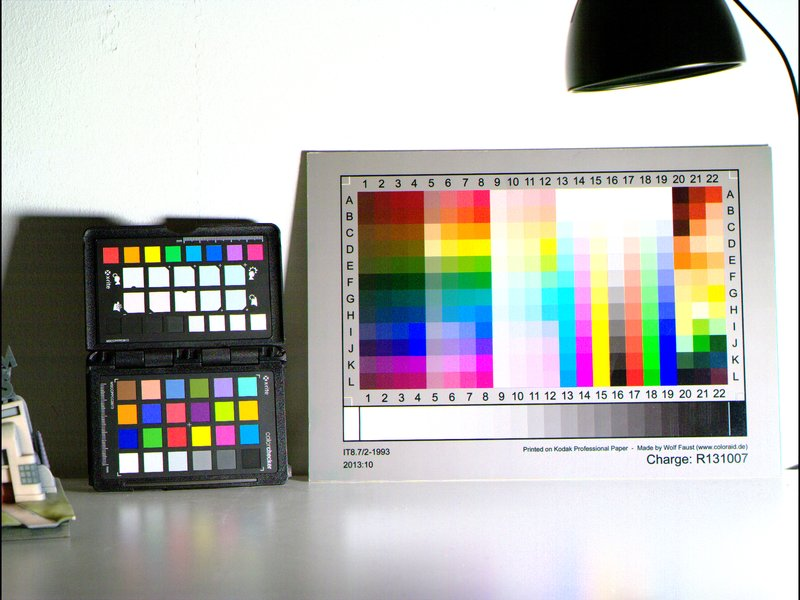
\includegraphics[height=5cm]{images/10ms+4-fixrn-small}
\end{center}

Corrected with \importantKeyword{--rnfilter=2}

\begin{center}
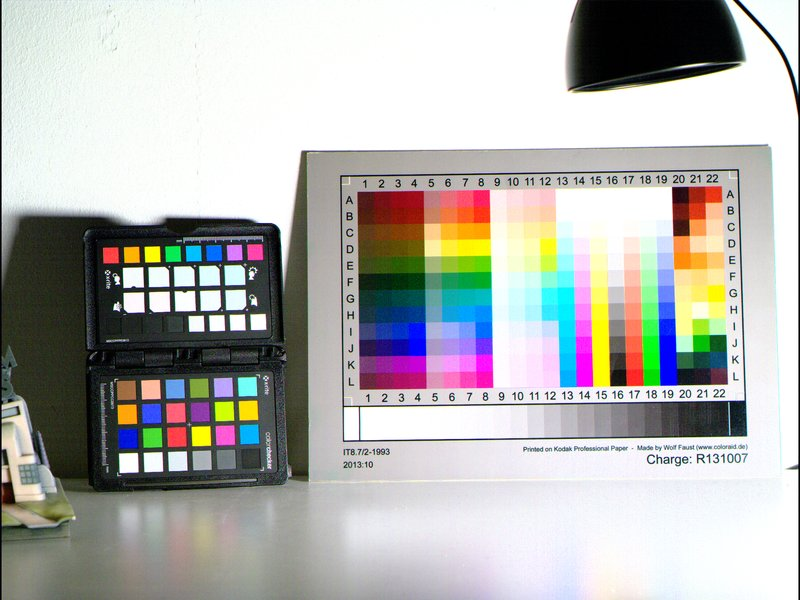
\includegraphics[height=5cm]{images/10ms+4-rnfilter2-small}
\end{center}

Larger images (half-res): 

- 10ms+4-no-blackcol.jpg - \href{http://files.apertus.org/AXIOM-Beta/snapshots/pattern-noise/10ms+4-no-blackcol.jpg}{http://files.apertus.org/AXIOM-Beta/snapshots/pattern-noise/10ms+4-no-blackcol.jpg}
- 10ms+4.jpg - \href{http://files.apertus.org/AXIOM-Beta/snapshots/pattern-noise/10ms+4.jpg}{http://files.apertus.org/AXIOM-Beta/snapshots/pattern-noise/10ms+4.jpg}
- 10ms+4-fixrn.jpg - \href{http://files.apertus.org/AXIOM-Beta/snapshots/pattern-noise/10ms+4-fixrn.jpg}{http://files.apertus.org/AXIOM-Beta/snapshots/pattern-noise/10ms+4-fixrn.jpg}
- 10ms+4-rnfilter2.jpg - \href{http://files.apertus.org/AXIOM-Beta/snapshots/pattern-noise/10ms+4-rnfilter2.jpg}{http://files.apertus.org/AXIOM-Beta/snapshots/pattern-noise/10ms+4-rnfilter2.jpg} 

\href{http://files.apertus.org/AXIOM-Beta/snapshots/pattern-noise/10ms+4-no-blackcol.jpg}{10ms+4-no-blackcol.jpg}\\
\href{http://files.apertus.org/AXIOM-Beta/snapshots/pattern-noise/10ms+4.jpg}{10ms+4.jpg}\\
\href{http://files.apertus.org/AXIOM-Beta/snapshots/pattern-noise/10ms+4-fixrn.jpg}{Final10ms+4-fixrn.jpg}\\
\href{http://files.apertus.org/AXIOM-Beta/snapshots/pattern-noise/10ms+4-rnfilter2.jpg}{10ms+4-rnfilter2.jpg}\\

All files used for this test, including scripts, calibration frames and uncompressed images, can be found here: \href{http://files.apertus.org/AXIOM-Beta/snapshots/pattern-noise/}{here}.

\href{http://files.apertus.org/AXIOM-Beta/snapshots/pattern-noise/10ms.raw12Raw12}{image: 10ms.raw12}\\
\href{http://files.apertus.org/AXIOM-Beta/snapshots/pattern-noise/darkframe-x1.pgm}{Calibration frames: darkframe-x1.pgm} and \href{http://files.apertus.org/AXIOM-Beta/snapshots/pattern-noise/dcnuframe-x1.pgm}{dcnuframe-x1.pgm}\\
\href{http://files.apertus.org/AXIOM-Beta/snapshots/pattern-noise/10ms.DNG}Final image (--rnfilter=2): {10ms.DNG}\\
\href{http://files.apertus.org/AXIOM-Beta/snapshots/pattern-noise/fpntest.sh}{Testing script: fpntest.sh}\\
\href{http://files.apertus.org/AXIOM-Beta/snapshots/pattern-noise/fpntest.log}{Script output: fpntest.log}\\





 

\subsection{Matrix Color Conversion} %See also mat4_conf.sh









\subsection{CMV12000 PLR}
\subsection{CMV12000 Response Curves}